\begin{figure}[h]
	\centering
	\begin{subfigure}{0.31\textwidth}
		\centering
		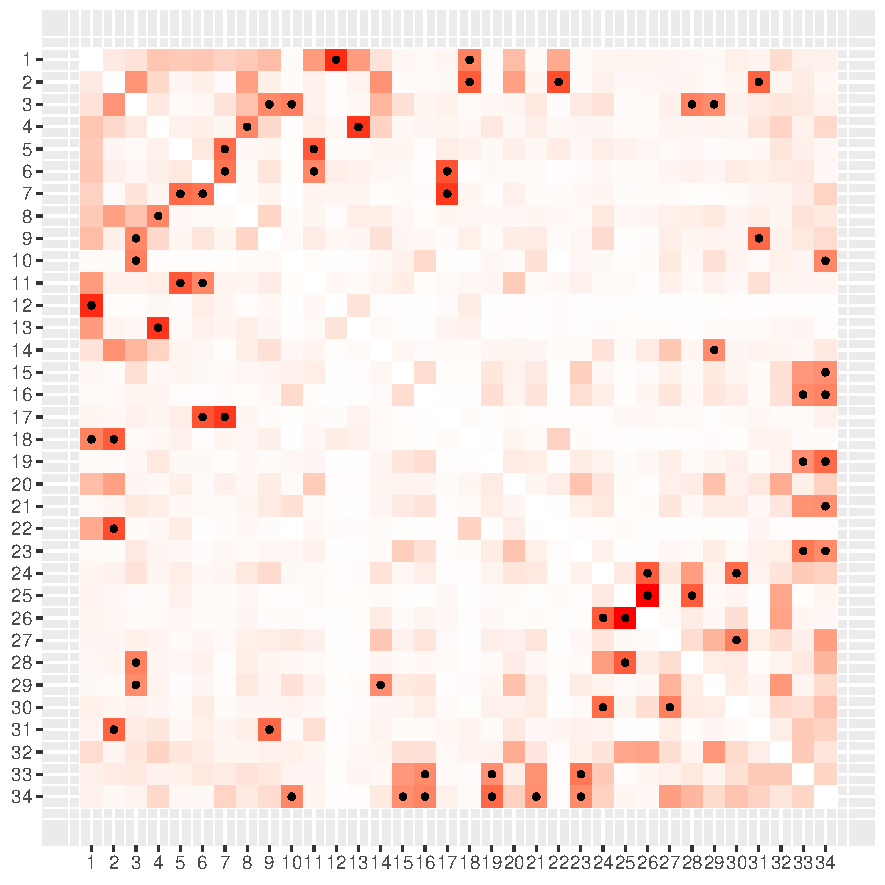
\includegraphics[width=\textwidth]{figures/K10-posterior-W.pdf}
		\caption{K10 ($T: 15$)}
	\end{subfigure}
	\begin{subfigure}{0.31\textwidth}
		\centering
		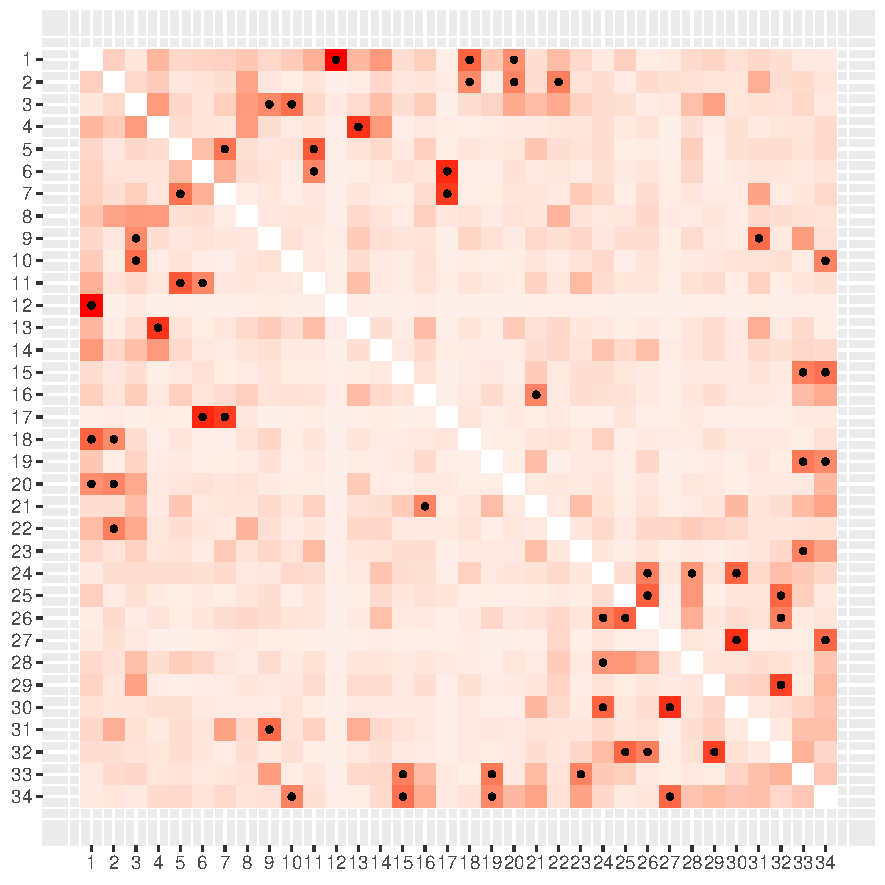
\includegraphics[width=\textwidth]{figures/K11-posterior-W.pdf}
		\caption{K11 ($T: 12$)}
	\end{subfigure}
	\begin{subfigure}{0.31\textwidth}
		\centering
		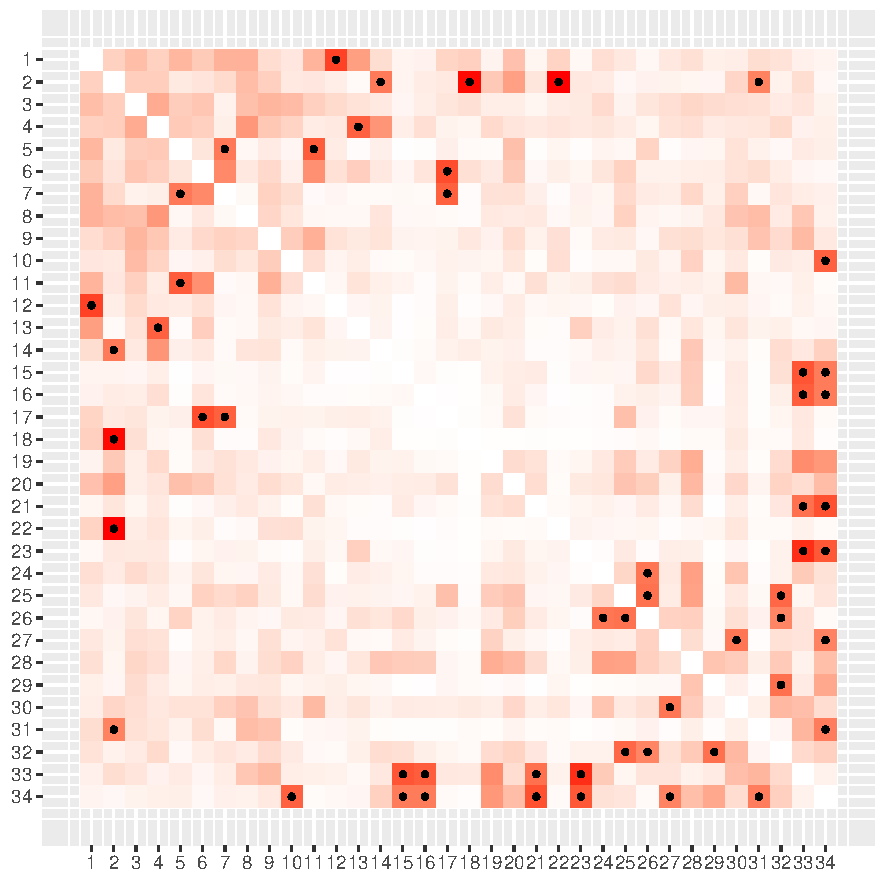
\includegraphics[width=\textwidth]{figures/K12-posterior-W.pdf}
		\caption{K12 ($T: 10$)}
	\end{subfigure}
	\begin{subfigure}{0.31\textwidth}
		\centering
		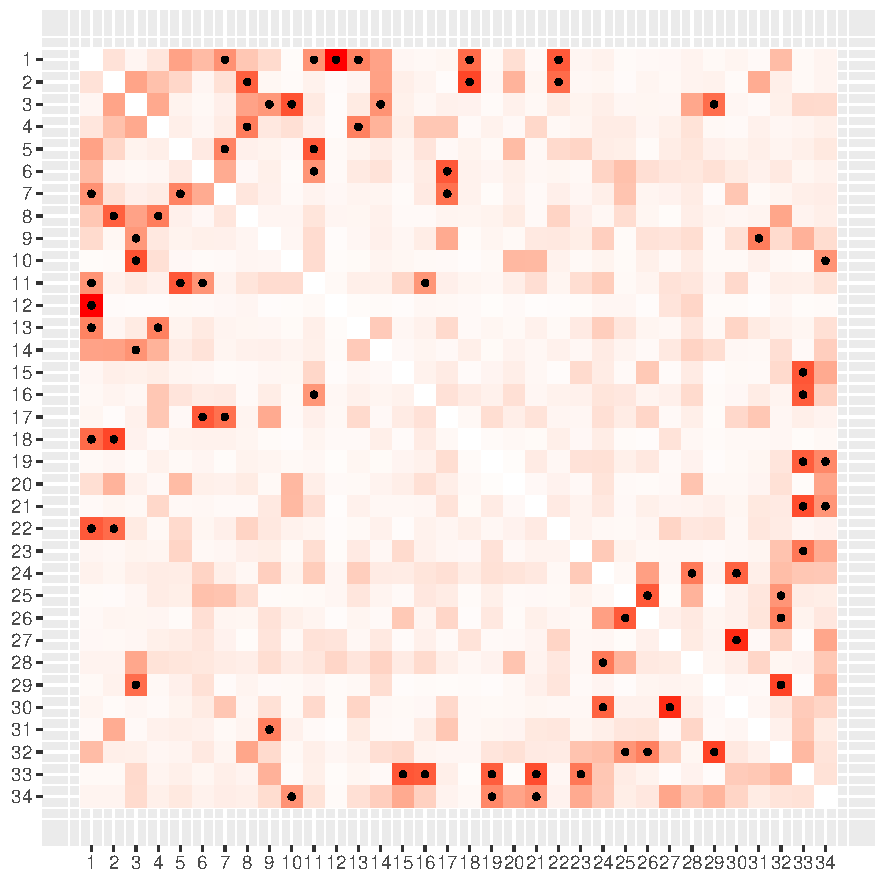
\includegraphics[width=\textwidth]{figures/K20-posterior-W.pdf}
		\caption{K20 ($T: 15$)}
	\end{subfigure}
	\begin{subfigure}{0.31\textwidth}
		\centering
		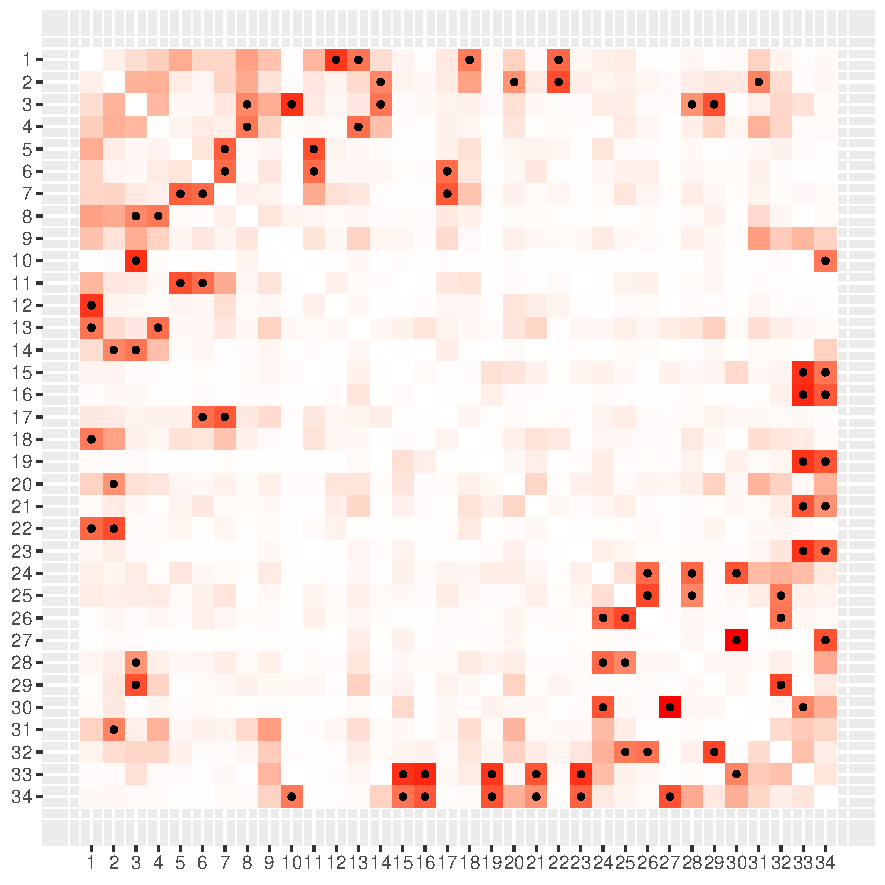
\includegraphics[width=\textwidth]{figures/K21-posterior-W.pdf}
		\caption{K21 ($T: 12$)}
	\end{subfigure}
	\begin{subfigure}{0.31\textwidth}
		\centering
		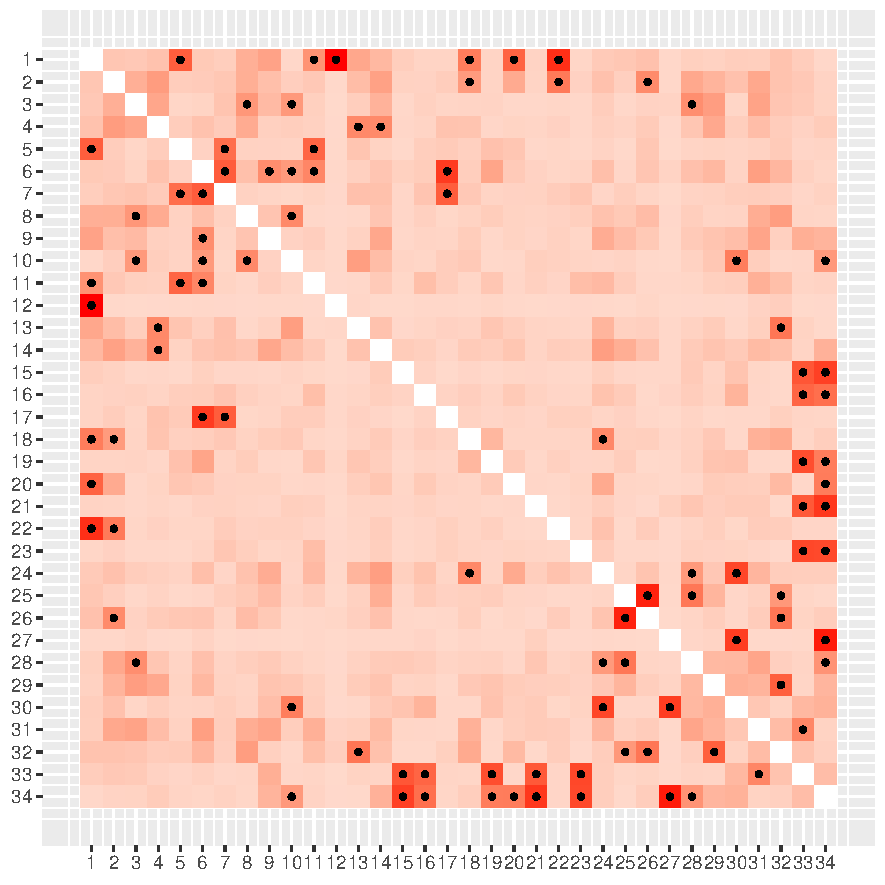
\includegraphics[width=\textwidth]{figures/K22-posterior-W.pdf}
		\caption{K22 ($T: 10$)}
	\end{subfigure}
	\caption{Posterior Adjacency Matrices.}
	\label{fig:K1}
\end{figure}
